\section{Introduction}
\label{sec:intro}
\begin{figure}[!h]
    \centering
    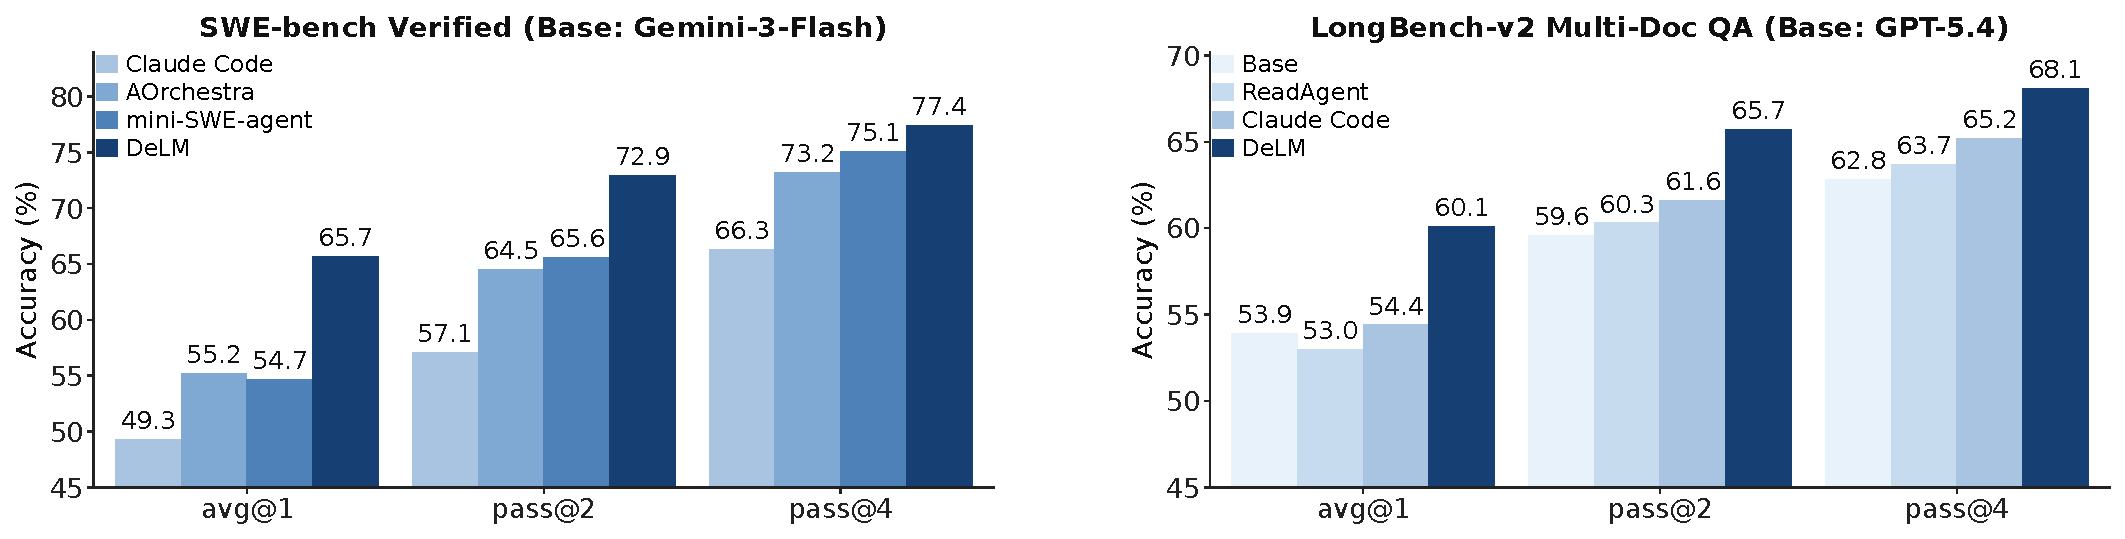
\includegraphics[width=1\linewidth]{teaser.pdf}
    \caption{\textbf{Comparison on SWE-bench Verified and LongBench-v2 Multi-Doc QA.} Our method, \toolName{}, achieves the best average performance across both agentic and long-context benchmarks.}
    \label{fig:placeholder}
\end{figure}


Multi-agent systems (MAS) offer a natural way to scale large language model reasoning at test time. Instead of relying on a single model invocation to solve a complex task end-to-end, MAS decompose the problem into subtasks, dispatch multiple agents in parallel, and aggregate their intermediate progress~\citep{hong2023metagpt, feng2026agentswing, ruan2026aorchestra, zhang2025recursive, openai_codex_2025, anthropic_claude_code_2026, team2026kimi}. This paradigm is increasingly important in two representative settings. The first is test-time scaling, where multiple agents can explore different hypotheses or pursue alternative reasoning paths in parallel while still sharing intermediate progress. The second is long-context reasoning, such as multi-document question answering, where agents can process different evidence clusters concurrently. In both cases, the value of MAS is not simply to issue more model calls, but to convert additional test-time computation into useful parallel progress. These two settings also capture core challenges in emerging automated research workflows~\citep{liu2026skydiscover,alphaevolve2025}, where agents must both scale exploration across hypotheses and reason over large collections of papers, code, experiments, and intermediate findings.
\begin{figure}
    \centering
    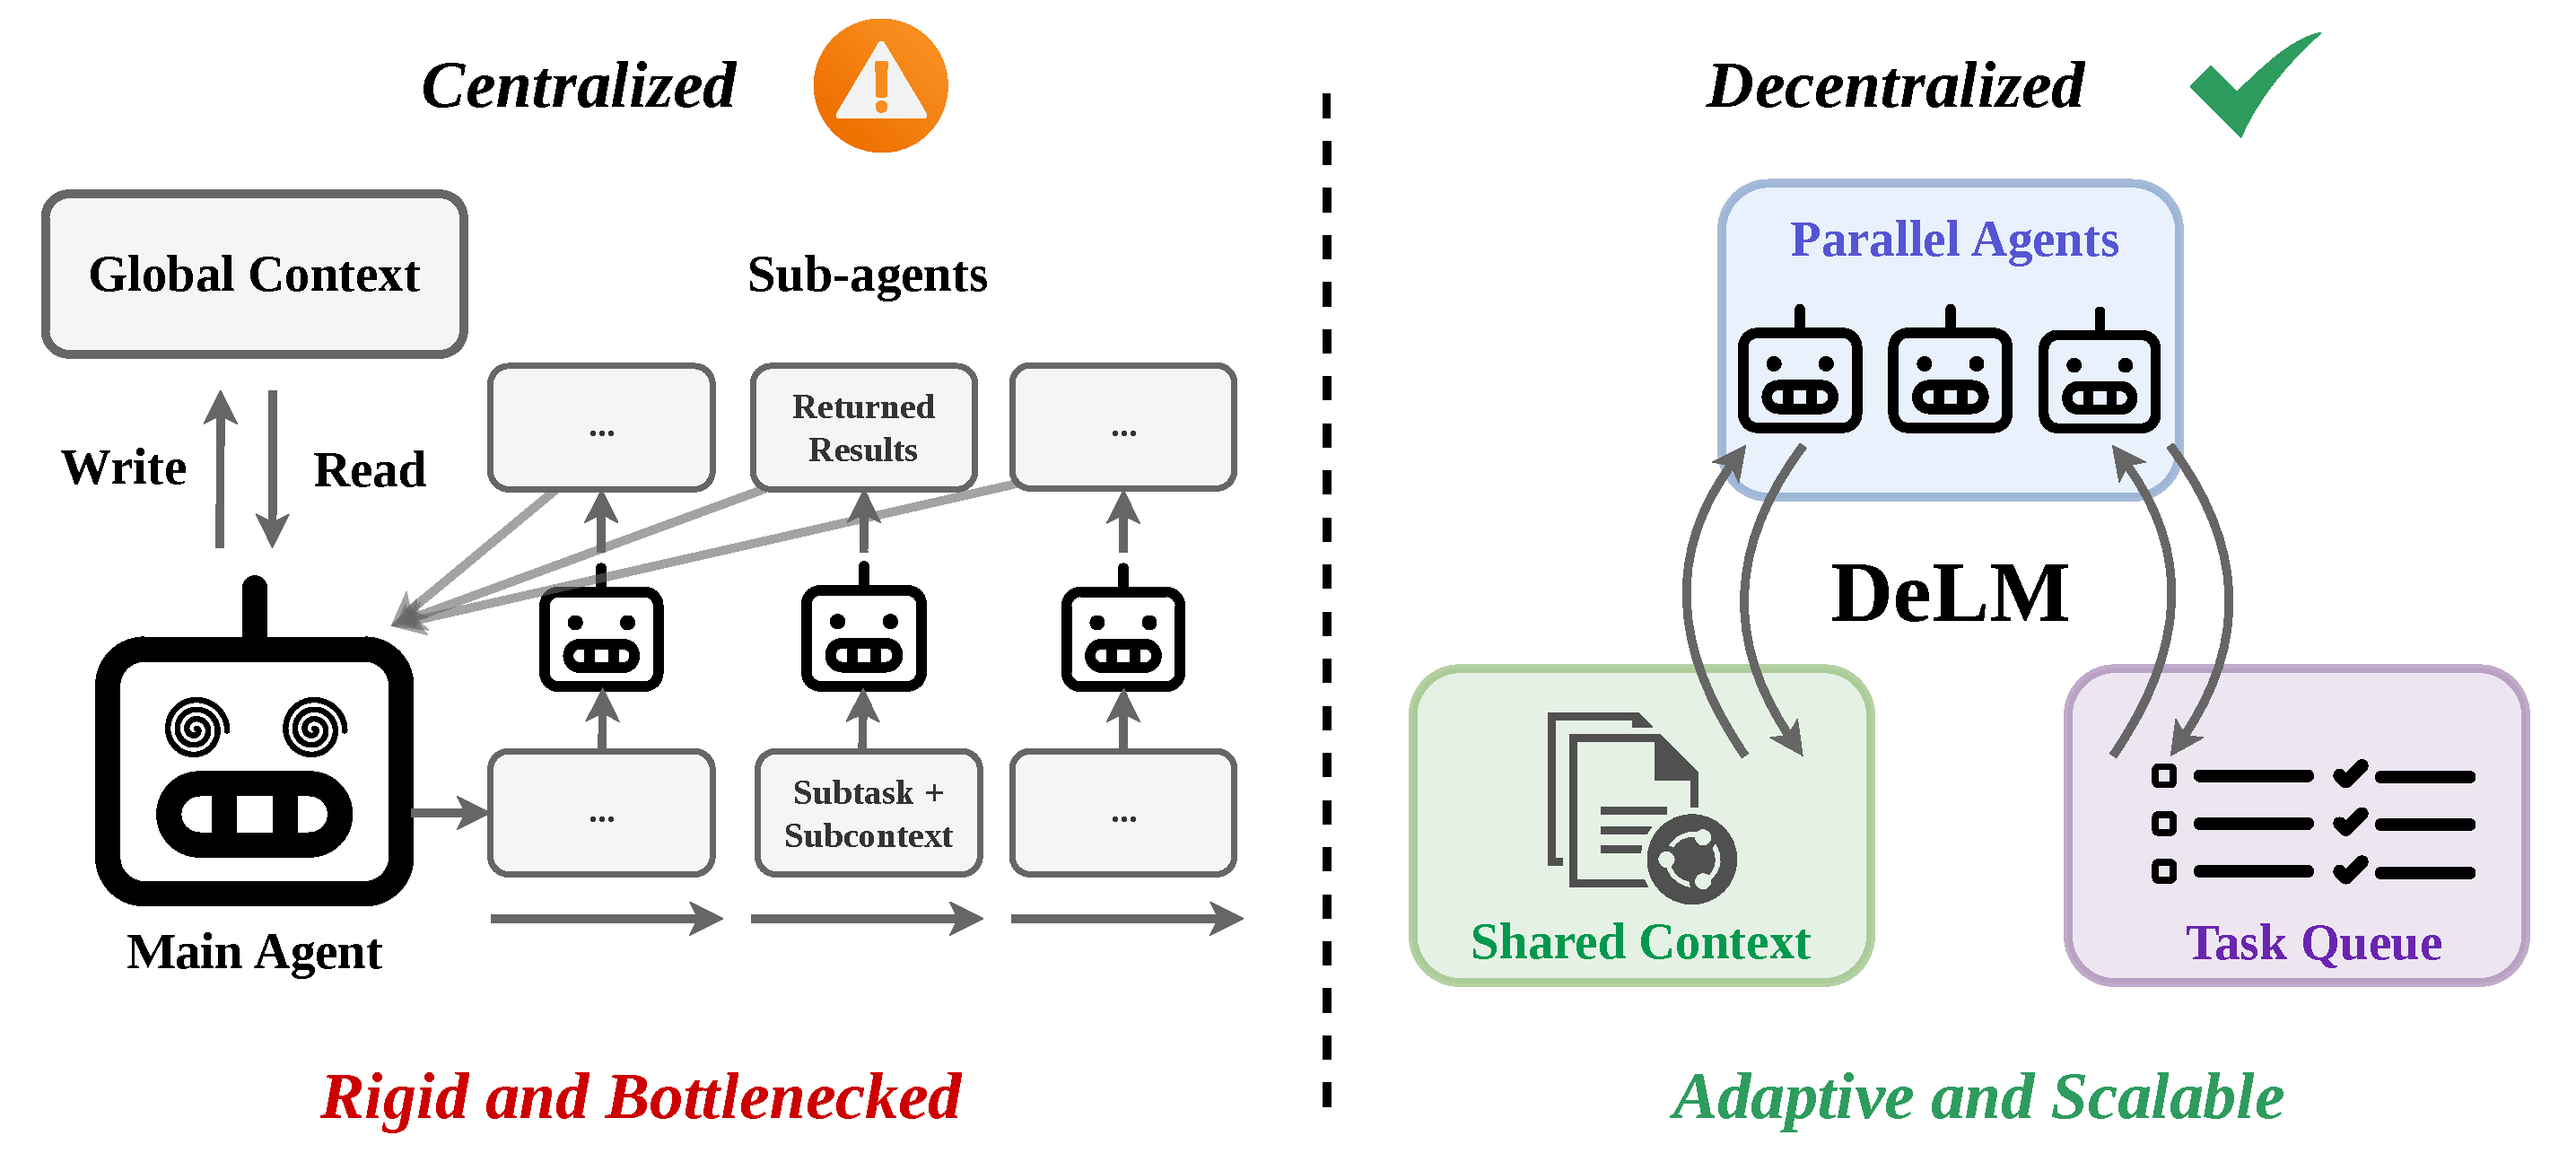
\includegraphics[width=1\linewidth]{first.pdf}
    \caption{
\textbf{Centralized vs. decentralized multi-agent systems.} Centralized MAS relies on a main agent to assign subcontexts, spawn sub-agents, and integrate returned results through a synchronous scatter--gather loop, creating a bottleneck where progress is gated by both the central merge step and the slowest worker. In contrast, \toolName{} decentralizes coordination through parallel agents, a shared context, and a task queue, allowing agents to exchange progress through shared state, asynchronously claim ready tasks, and scale more adaptively as the number of subtasks grows.
}
    \label{fig:first}
\end{figure}


Realizing this potential, however, depends critically on how agents coordinate. Most existing MAS frameworks, including Claude Code Subagents~\citep{anthropic_claude_code_2026}, Kimi Agent Swarm~\citep{team2026kimi}, and AOrchestra~\citep{ruan2026aorchestra}, rely on centralized orchestration: a main agent decomposes the problem, assigns subtasks and corresponding subcontexts to sub-agents, waits for their outputs, and then integrates the results or launches another round of subtasks, as illustrated in Figure~\ref{fig:first} (left). 
The limitation is that centralized MAS parallelize sub-agent execution, but not the coordination around it.
In test-time scaling, the benefit of additional agents depends on whether useful progress can be shared across workers efficiently and faithfully. Centralized orchestration weakens this benefit in two ways. First, it scales poorly: every useful finding, failure, or partial solution must return to the main agent, which then decides how to merge and broadcast that information to other sub-agents. As the number of agents grows, progress sharing becomes a serialized communication bottleneck. Second, during this routing process, the main agent may dilute, omit, or distort useful details, causing important progress to be lost. We provide a more detailed analysis in Section~\ref{sec:swe_analyze}. This bottleneck also arises in long-context reasoning: the main agent must pre-assign evidence clusters to sub-agents, often before knowing which evidence is relevant or how different pieces should be combined~\citep{anthropic_claude_code_2026, zhang2025recursive}. If a sub-agent receives insufficient context, it return control to the main agent, triggering additional retrieval or another delegation round. As subtasks or evidence clusters grow, this back-and-forth makes coordination slower, more iterative, and increasingly constrained by a single overloaded main agent.

To address these bottlenecks, we propose Decentralized Language Models (\toolName{}), a MAS framework that shifts coordination from a central controller to a shared problem state. As shown in Figure~\ref{fig:first} (right), \toolName{} is built around three core components: parallel agents, a shared context, and a task queue. Rather than routing every interaction through a main agent, agents asynchronously draw tasks from the queue, read accumulated progress from the shared context, perform local reasoning, and write back compact verified updates. This design also differs from peer-to-peer communication, where agents exchange messages directly. Instead, \toolName{} uses the verified shared context as a common communication substrate: once an update is admitted, it becomes visible to all agents as reusable problem state. As a result, \toolName{} supports both motivating settings: in test-time scaling, useful findings, failures, and partial solutions can propagate through shared context rather than being repeatedly merged and rebroadcast by a main agent. In long-context reasoning, agents can process different evidence clusters concurrently while maintaining a compact global view of the corpus and accumulated evidence.
\begin{keyidea}
\textbf{Key idea.} Unlike existing MAS, which rely on a central controller and synchronous scatter--gather coordination, \toolName{} lets agents coordinate asynchronously through a shared, verified context. Agents claim tasks from a queue and write back compact, verified results as they finish, making progress visible to all workers without requiring a main agent to merge, filter, and rebroadcast it.
\end{keyidea}

We evaluate \toolName{} in three settings that stress different forms of multi-agent coordination: (1) software-engineering test-time scaling on SWE-bench Verified~\citep{jimenez2024swebench}, which stresses parallel exploration across different reasoning trajectories; (2) long-context multi-document QA on LongBench-v2~\citep{bai2025longbench}, which stresses within-task parallelism as agents concurrently inspect different evidence clusters; and (3) aggregation-heavy long-context reasoning on OOLONG~\citep{bertsch2025oolong}, which highlights the complementarity between \toolName{}’s decentralized verified context and the code-mediated execution of RLM~\citep{zhang2025recursive}. Our key findings are: 
\begin{itemize}
    \item \textbf{\toolName{} converts parallel software-engineering attempts into shared exploration.} On SWE-bench Verified (\S~\ref{sec:swe}), as shown in Table~\ref{tab:swebench_verified}, \toolName{} achieves the strongest performance across test-time scaling metrics, reaching 77.4\% pass@4 while reducing cost to \$0.12 per task which is only roughly half of the baselines. Section~\ref{sec:swe_analyze} further explains these gains through trace-level examples showing how compact shared context helps agents reuse discoveries.
    \item \textbf{\toolName{} enables iterative shared-state reasoning over long contexts.} On LongBench-v2 (\S~\ref{sec:longbench}), as shown in Table~\ref{tab:multidoc_results}, \toolName{} achieves the highest average accuracy across four frontier models, improving over the best baseline by up to 5.7 percentage points. Section~\ref{sec:longbench_ablation} further shows that both admission-time verification and hierarchical summarization contribute to these gains.
    \item \textbf{\toolName{} acts as a coordination layer for programmatic reasoning systems.} On OOLONG (\S~\ref{sec:with_rlm}), as shown in Table~\ref{tab:oolong}, vanilla \toolName{} underperforms RLM because the benchmark requires exact row-level aggregation, where code-mediated execution is especially useful; however, combining RLM with \toolName{} yields the best accuracy and lowest cost, showing that \toolName{} extends beyond conversational agents to code-based reasoning workflows.
\end{itemize}

\section{Motivation and Design Principles}
\label{sec:motivation}

\subsection{From Prompt Routing to Shared State}

Section~\ref{sec:intro} identifies centralized coordination as a bottleneck in existing MAS. Here, we refine this observation by focusing on its communication mechanism. Centralized MAS are largely {prompt-routed}: intermediate progress is passed through the main agent, rewritten into subsequent prompts, and selectively exposed to other agents. Thus, parallel execution does not by itself guarantee parallel progress sharing.

This perspective motivates a different communication substrate. Instead of repeatedly encoding coordination decisions into prompts, \toolName{} makes intermediate progress persistent: agents write compact, verified updates into a shared context that later agents can read directly. Coordination therefore becomes {state-based}, with useful findings, failures, and constraints accumulating as shared problem state rather than passing through a central controller.

\subsection{Compact, Global, Unfoldable Shared Context}

State-based communication is useful only if the shared context remains usable as the problem grows. Sharing raw documents or full agent traces preserves maximal information, but quickly overwhelms each agent's context window and increases cost. Sharing only compact summaries is cheaper, but risks losing details, qualifications, or cross-document evidence needed for reliable reasoning.

\toolName{} addresses this trade-off with an unfolding mechanism. Agents read highly compact gists by default and selectively expand them into detailed summaries or raw evidence when needed. This coarse-to-fine access pattern enables coordination over the full problem while incurring detailed inspection costs only for relevant evidence.


\subsection{Verified Before Admission}

Because the shared context serves as the communication substrate for all agents, errors in this state can propagate widely. Once admitted, an unsupported claim may become reusable problem state, misleading later agents and shaping downstream reasoning. Post-hoc answer checking is insufficient, because such errors may have already influenced intermediate decisions.

\toolName{} mitigates this risk through admission-time verification. Before an update is added to the shared context, it is checked against its underlying evidence, including source context and reasoning trajectories. Unsupported or distorted updates are rejected or regenerated, turning the shared context from a raw message buffer into curated shared state.
